\question[10] Completa las afirmaciones de acuerdo con la información que presenta la gráfica de la figrua \ref{fig:dist_tiempo_01}.

\begin{minipage}[t]{0.35\linewidth}
    \begin{figure}[H]
        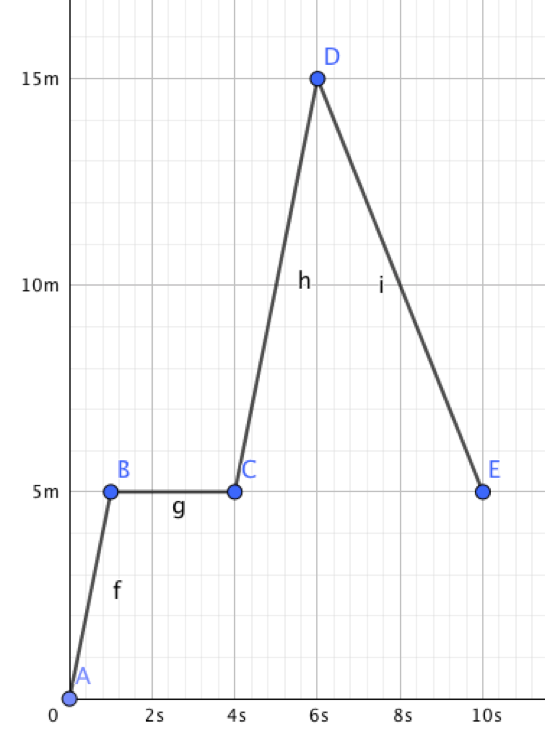
\includegraphics[width=\linewidth]{Images/dist_tiempo_01}
        \caption{La gráfica representa el desplazamiento de un atleta durante su entrenamiento.}
        \label{fig:dist_tiempo_01}
    \end{figure}
\end{minipage}%
\begin{minipage}[t]{0.65\linewidth}
    \begin{parts}
        {\printanswers
            \subfile{Questions/Parts/question005a}
        }
        \subfile{Questions/Parts/question005b}
        \subfile{Questions/Parts/question005c}
        \subfile{Questions/Parts/question005d}
    \end{parts}
\end{minipage}
